\chapter{Návrh aplikace}
    Návrh aplikace je velice důležitou fází projektu, ve které by mělo dojít ke sjednocení požadavků zadavatelů a reálného provedení. Vytvořením dobrého návrhu se zamezí případným kolizím a zároveň proběhne první interakce mezi zákazníkem a dodavatelem. Ze strany UČL byl vznesen požadavek, aby aplikace byla snadno ovladatelná a měla moderní vzhled. Databázové schéma bylo čistě na našem rozhodnutí.
    
    \section{Wireframy}
        Jednou z nejdůležitějších sekcí bylo navrhnout, jak budou jednotlivé stránky vypadat a kolik jich aplikace bude obsahovat. Základní rozložení stránek bylo na mém rozhodnutí, nicméně musel jsem dodržet požadavky UČL AV. Design měl být jednoduchý, uživatelsky přívětivý a moderní. Tyto návrhy musely být a byly schváleny pracovníky UČL AV.
        
        Grafika měla být jednoduchá, bez složitých a obsáhlých prvků. Pro návrh GUI jsem se rozhodl použít webovou aplikaci Moqups\footnote{domovská stránka: \url{https://moqups.com/}}. Její bezplatná verze nabízí obrovské množství šablon pro grafické návrhy. Od základních prvků jako je tlačítko nebo nadpis, po mírně složitější formuláře. Pro snadnější a moderní stylování aplikace jsem chtěl použít Bootstrap, a proto je velikou výhodou, že Moqups má bootstrapovské prvky v nabídce. 
        
        \subsection{Login}
            Pro úvodní přihlašovací stránku jsem vybral jednoduchý formulář, ve kterém je email a heslo, viz obrázek \ref{fig:login}. Pozadí, které by se dalo v budoucím rozšíření měnit, je jako na všech ostatních stránkách bílé.
            
        \subsection{Hlavní stránka}
            Po úspěšném přihlášení do aplikace se zobrazí hlavní stránka, která je rozdělena do tří částí, jak je vidět na obrázku \ref{fig:main}. V hlavičce se nachází společně s nadpisem odkaz na seznam autorů a vydavatelů děl a dropwdown s možnostmi uživatele. Dále je zde filtr aplikovatelný na zobrazená díla. Zadání vyžadovalo vyhledat elektronickou literaturu podle autora, roku vydání, textu obsaženého v díle a statusu. Třetí část obsahuje samotný seznam děl. Tento seznam je ve tvaru tabulky se sloupci název díla, autor, rok vydání, status, odkaz na přílohy a nezbytné akce a navíc se dá tabulka seřadit podle sloupců. U seznamu děl lze nastavit počet zobrazených děl a obsahuje rychlý vyhledávač textu.

        \subsection{Metadata}
            Na obrázku \ref{fig:metadata} je vidět rozložení stránky pro úpravu metadat. Opět se skládá ze tří částí. První obsahuje navigaci, dropdown pro přihlášeného uživatele a nadpis. Druhá část je věnována autorům a vydavatelům. V tomto oddílu bude umožněno přidávat a odebírat autora nebo vydavatele. Poslední sekce obsahuje formulář pro úpravu metadat literárního díla. Společně s pracovníky UČL AV byly vybrány nejdůležitější atributy, které je zde možno upravit. 
        
        \subsection{Přílohy}
            Součástí zadání práce je správa příloh, zejména fotografií. Úkolu je věnován právě tento segment. Obsahem wireframu přílohy jsou naskenované jednotlivé stránky daného literárního díla. V horní části se opět objevuje navigace, uživatelské funkce a nadpis viz \ref{fig:attachments}. Následuje sekce věnovaná hromadnému uploadu skenů do níže zobrazené fotogalerie.
            
        \subsection{Autoři a vydavatelé}
            Pro správu autorů a vydavatelů byl použit návrh zobrazený v příloze \ref{fig:authPub}. V horní části se vyskytuje navigace, nezbytné funkce a nadpis. Dále je zde umístěna tabulka záznamů, ve kterých lze snadno vyhledávat. Každý záznam lze upravit a smazat. Pro upravení záznamu byl navržen wireframe \ref{fig:edit}, který obsahuje navigaci, funkce a zjednodušený formulář. Formuláře pro upravení vydavatele nebo autora jsou totožné.
            
            \begin {figure}[H]\centering
                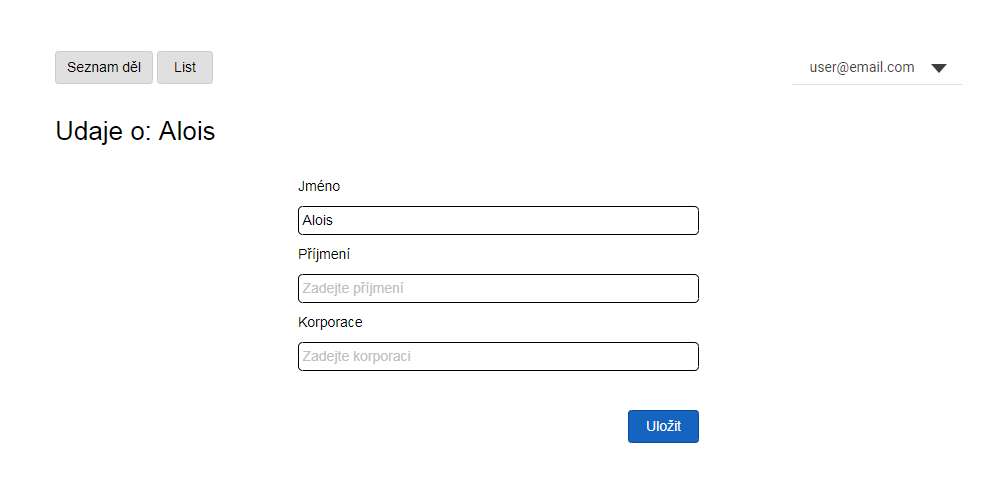
\includegraphics[width=\textwidth]{images/edit}
                \caption {Úprava autora}
                \label {fig:edit}
            \end{figure}
            
        \subsection{Text}
            Nejdůležitějším prvkem aplikace byla bezesporu možnost upravovat text literárního díla. Pro tuto funkci byla navržena stránka \ref{fig:text}. Jako u předešlých wireframů, horní část se věnuje navigaci, funkcím uživatele a nadpisu. Dále je vidět rozložení stránky na dva oddíly. Jeden pro text knihy a druhý pro možnost vkládání značek. Menu vpravo bylo navrženo vzhledem k nadměrné velikosti první části tak, aby bylo viditelné, když se uživatel posune níž.
            
    \section{Databázové schéma}
        Neméně duležitou součástí projektu byla databáze. Ze strany UČL AV nebyly vzneseny žádné požadavky na podobu databáze, proto se mohlo schéma přizpůsobit dle potřeby aplikace.
        
    \section{Autentizace}
        jak je zabezpečené heslo uživatele
